\chapter{More LaTeX Patterns}
\label{app:more-patterns}

% This second optional appendix collects further patterns: subfigures, logic
% notation, units, abbreviations, and a landscape page. Each pattern relies on
% a package already loaded in preamble.tex. Keep what the thesis uses and
% delete the rest, together with its package.

\section{Subfigures and side-by-side floats}

Use \texttt{subcaption} when several panels share one figure number. Each panel
keeps its own caption, and \cref{fig:subfigures} can be cited as a whole or panel
by panel: \cref{fig:subfigure-graph} shows the input and
\cref{fig:subfigure-workflow} the computation.

\begin{figure}[htbp]
  \centering
  \begin{subfigure}[b]{0.46\linewidth}
    \centering
    \begin{tikzpicture}[
  vertex/.style={circle,draw=LMFINavy,thick,minimum size=8mm,inner sep=0pt},
  edge/.style={-{Stealth[length=2.4mm]},thick,LMFITeal},
  node distance=2.2cm
]
  \node[vertex] (a) {$a$};
  \node[vertex, right=of a] (b) {$b$};
  \node[vertex, right=of b] (c) {$c$};
  \node[vertex, below=1.0cm of c] (d) {$d$};

  \draw[edge] (a) -- (b);
  \draw[edge] (b) -- (c);
  \draw[edge] (c) -- (d);
  \draw[edge] (a) to[bend right=18] (d);
\end{tikzpicture}

    \caption{Input graph.}
    \label{fig:subfigure-graph}
  \end{subfigure}\hfill
  \begin{subfigure}[b]{0.46\linewidth}
    \centering
    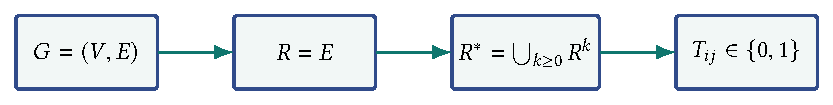
\includegraphics[width=\linewidth]{figures/example-workflow.pdf}
    \caption{Computation.}
    \label{fig:subfigure-workflow}
  \end{subfigure}
  \caption{Two views of the running example.}
  \label{fig:subfigures}
\end{figure}

A figure and a table can also share one row. Put each in a \texttt{minipage} and
name them with \verb|\captionof|, as in \cref{fig:side-graph,tab:side-edges}.

\begin{figure}[htbp]
  \centering
  \begin{minipage}[c]{0.46\linewidth}
    \centering
    \begin{tikzpicture}[
  vertex/.style={circle,draw=LMFINavy,thick,minimum size=8mm,inner sep=0pt},
  edge/.style={-{Stealth[length=2.4mm]},thick,LMFITeal},
  node distance=2.2cm
]
  \node[vertex] (a) {$a$};
  \node[vertex, right=of a] (b) {$b$};
  \node[vertex, right=of b] (c) {$c$};
  \node[vertex, below=1.0cm of c] (d) {$d$};

  \draw[edge] (a) -- (b);
  \draw[edge] (b) -- (c);
  \draw[edge] (c) -- (d);
  \draw[edge] (a) to[bend right=18] (d);
\end{tikzpicture}

    \captionof{figure}{The example graph.}
    \label{fig:side-graph}
  \end{minipage}\hfill
  \begin{minipage}[c]{0.40\linewidth}
    \centering
    \begin{tabular}{cc}
      \toprule
      From & To \\
      \midrule
      $a$ & $b$ \\
      $b$ & $c$ \\
      $c$ & $d$ \\
      $a$ & $d$ \\
      \bottomrule
    \end{tabular}
    \captionof{table}{Its edge list.}
    \label{tab:side-edges}
  \end{minipage}
\end{figure}

\section{Logic and computer-science notation}

Project macros live in \texttt{macros.tex}: \verb|\N|, \verb|\Reach| and a
semantic-bracket delimiter \verb|\sem|. With them,
\[
  \Reach(u) = \{\, v\in V \mid u\mathrel{R^*}v \,\}, \qquad
  \sem{\varphi}_G \subseteq V, \qquad
  \bigl|\Reach(u)\bigr| \leq n \in \N .
\]
The \texttt{mathpartir} package typesets inference rules; here are the
introduction and elimination rules of implication, in a sequent style used in
logic courses:
\begin{mathpar}
  \inferrule*[right=$\to$I]{\Gamma, A \vdash B}{\Gamma \vdash A \to B}
  \and
  \inferrule*[right=$\to$E]{\Gamma \vdash A \to B \\ \Gamma \vdash A}{\Gamma \vdash B}
\end{mathpar}
Commutative diagrams use \texttt{tikz-cd}. The square below commutes because
every edge lies in the closure: both paths from $E$ to $V\times V$ are the
inclusion of $E$.
\[
  \begin{tikzcd}[column sep=large]
    E \arrow[r, hook] \arrow[d, hook] & R^* \arrow[d, hook] \\
    V\times V \arrow[r, equal] & V\times V
  \end{tikzcd}
\]

% Document each notation macro in macros.tex, and define only those that
% recur. For named functions, declare an operator (\DeclareMathOperator)
% instead of using plain italic letters.

\section{Units, quotations, and footnotes}

\texttt{siunitx} formats numbers and units consistently in the language of the
thesis. The triple loop of \cref{alg:warshall} performs \num{1073741824} Boolean
updates for $n=\num{1024}$; at \qty{1.5}{\giga\hertz} and one update per cycle,
that takes about \qty{0.72}{\second}. Quotations use \texttt{csquotes}:
\enquote{a quotation may contain \enquote{a nested quotation}}, with the quotation
marks of the active language. A footnote\footnote{Footnotes number continuously
within a chapter and are set at the bottom of the page.} stays out of the main
argument.

\section{Abbreviations}

The \texttt{acro} package expands an abbreviation at its first use and shortens
it afterwards. A \ac{dag} has no directed cycle, whereas every vertex of a
\ac{scc} reaches every other; a \ac{dag} is therefore the opposite extreme. Later
mentions give only \ac{dag} and \ac{scc}. Declare abbreviations in
\texttt{macros.tex}; the list below is produced by \verb|\printacronyms|.

\printacronyms[heading=none]

\section{Cross-references}

Write \verb|\cref| inside a sentence, as in \cref{tab:side-edges}, and
\verb|\Cref| at the start of one: \Cref{fig:subfigures} is such a case. Several
objects of one type can be joined: \cref{fig:subfigures,fig:side-graph}. Give every label a short prefix
(\texttt{fig:}, \texttt{tab:}, \texttt{eq:}, \texttt{thm:}) and cite only objects
that the text discusses.

\clearpage
\begin{landscape}
\section{A wide table on a landscape page}

A table that is too wide for the text block can be placed on a rotated page with
\texttt{pdflscape}; viewers show the page rotated, as does the printed copy.
\Cref{tab:landscape} lists the size of the Boolean matrix and the number of
updates of the triple loop for growing graphs.

\begin{table}[htbp]
  \centering
  \caption{Matrix entries and Boolean updates of \cref{alg:warshall} for $n$ vertices.}
  \label{tab:landscape}
  \small
  \begin{tabular}{@{}l *{9}{r}@{}}
    \toprule
    $n$ & \num{4} & \num{8} & \num{16} & \num{32} & \num{64} & \num{128} & \num{256} & \num{512} & \num{1024} \\
    \midrule
    Entries $n^2$ & \num{16} & \num{64} & \num{256} & \num{1024} & \num{4096} & \num{16384} & \num{65536} & \num{262144} & \num{1048576} \\
    Updates $n^3$ & \num{64} & \num{512} & \num{4096} & \num{32768} & \num{262144} & \num{2097152} & \num{16777216} & \num{134217728} & \num{1073741824} \\
    \bottomrule
  \end{tabular}
\end{table}

% Use a landscape page only when a table or figure cannot be made legible in
% portrait: shrink the font or split the table first. Every landscape object
% needs the same caption and reference as any other float.
\end{landscape}
